%Existing Best Practices
\section{Related Work}
% Why Pronunciation is important
Pronunciation in second language acquisition (SLA) is interconnected with the building blocks of language-- grammar, vocabulary, and listening comprehension-- as well as integration into a language community. Thus, improving pronunciation leads to improvement in other areas of SLA and vice versa~\cite{sicola2015integrating,derwing2003esl}.  There are multiple ways that a first language (L1) of a speaker, usually a language spoken from a very young age, can interfere with acquiring sounds in a second language (L2). Sounds that distinguish meaning in an L1, called phonemes, may not distinguish meaning in an L2 or vice versa. As a result, interlocutors can be confused when communicating with an L2 speaker~\cite{rao2019key}. We discuss previous work that focuses on human- and computer- assisted methods for pronunciation improvement. 
% as well as work on designing visualizations for audio.  

%Past Research
%Non-tech
\subsection{Human-Mediated Pronunciation Training}
Little attention is given to pronunciation in textbooks and curricula other than at a collegiate level in the United States of America. This makes ad hoc reactive feedback for pronunciation common in foreign language classrooms from K-12~\cite{rao2019key,wei2006literature,darcy2021window}. Learners who receive ad hoc reactive feedback do not improve significantly in comparison with intentional methods of training. As a result, we leave this out of the discussion despite it being a common approach in classrooms~\cite{darcy2021window}. Beyond reactive feedback, three main methods of pronunciation instructor-dependent training are outlined below: reading out loud, mimicry of an L1 speaker, and minimal pair drills (drilling words that differ by one sound/phoneme\footnote{For example, hat/hit, fit/feet, cat/bat are minimal pairs in English. Hat and catch are not since they differ by more than one sound}).  

\subsubsection{Reading Out Loud}
\label{sec:reading}
A commonly studied method of pronunciation improvement is reading out loud~\cite{thomson_effectiveness_2015, chenRetAssist2024}. This can be achieved through paired practice, where peers listen and give feedback, mimicking practice, or group reading, where the whole classroom and teacher listen to the reader and provide feedback on pronunciation. The exercise improves oral reading fluency and reading comprehension~\cite{han2016integrating}, but is dependent on a teacher's input or practice with peers. Because feedback is given in real-time, L2 learners will not receive detailed pronunciation feedback.

\subsubsection{Mimicry of an L1 Speaker}
As mentioned in section \ref{sec:reading}, mimicry can be used in conjunction with reading out loud. It can also be used for shorter segments of pronunciation, such as words or sounds, which is the method we use in our study design. Research shows that mimicry is key in improving pronunciation~\cite{hinton_aptitude_2013, szyszka_good_2015}. While mimicry is used in classrooms, it does not require an active listener. L2 learners can practice mimicry with any kind of medium that includes audio, such as movies or podcasts, though this means they have to rely on their own judgment to adjust pronunciation. 

\subsubsection{Minimal Pair Drills}
\label{sec:minimal}
Minimal pair drills (MPDs) rely on listening and mimicking an L1 speaker to bring out the contrast that different sounds have by putting them in identical contexts. MPDs are used in speech therapy and language learning to great effect though they limit the context that sounds can appear based on the L1~\cite{barlow_minimal_2002, hamzah_teaching_2019, rahman_use_2018, brown_minimal_1995}. Despite potential downsides of minimal pairs, we contend that visually contrasting vowels will benefit the L2 learner.   

% Tech
\subsection{Computer-Assisted Pronunciation Training (CAPT)}
CAPT has the advantage over traditional pronunciation feedback by its ability to be used by many and be automatically catered to the individual. CAPT feedback takes two different forms: audio-only and visual accompanied by audio. The latter outperforms traditional and audio-only feedback~\cite{olson2014benefits,hew_effect_2004}. Visual feedback falls into two main categories: spectrograms and articulatory-based visualizations.

\subsubsection{Spectrograms} 
Spectrograms are useful for their flexibility in pronunciation feedback. They can be used to train vowels and consonants including the effects those sounds have on each other (Figure \ref{fig:specHeat}). Studies have shown the positive impact on pronunciation when students reflect on their speech with the aid of a spectrogram. But a spectrogram can require hours of training to correctly interpret and previous studies use it as a static tool instead of an interactive one~\cite{greene_recognition_1984}, likely because it is difficult to apply feedback. Using it as a static tool limits learners to reflect on their pronunciation without immediately adjusting their pronunciation. 

\subsubsection{Articulatory-based Visualizations}
Articulatory-based visualizations, on the other hand, are used in phonetic training to teach learners about articulators, such as the tongue and lips, in many different languages. Previous work focuses on two ABV: face-cutaway animations and vowel charts.

Animated face-cutaway diagrams display how articulators move during speech. Learners can view correct movement based on the animation and attempt to mimic the example speaker~\cite{bu2021pteacher}. However, this work does not display an animation of a learner's incorrect speech or how to change pronunciation from incorrect to be correct~\cite{bu2021pteacher}. As a result, feedback targets mistakes but does not provide feedback to move from current pronunciation to the target pronunciation.

Vowel charts display a vowel's location on a trapezoid. There are two ways to represent vowels on a vowel chart -- with IPA symbols (Figure \ref{fig:exampleVwlChart}) or with formants (Figure \ref{fig:freqVwlChart}). Previous studies show that vowel charts are effective within limited contexts in improving pronunciation ~\cite{paganus2006vowel,rehman2021real}. One method studied vowels by themselves while another limited it to vowel preceded by an 'h' and followed by a 'd'~\cite{paganus2006vowel,rehman2021real}. Both restrictions limit the real-world use of the tool. Furthermore, how learners understand what they see on an interactive vowel chart is unclear since all the studies interview participants in a reflexive way, making it difficult to know how to improve the interaction experience to facilitate a better understanding of a vowel chart. Finally, these vowel charts do not integrate the audio with the visual, requiring learners to listen and interpret visuals separately~\cite{paganus2006vowel,rehman2021real}.  

We designed a real-time interactive vowel chart system, \visowel{}, that would function for vowels in any context and provide integrated audio and visual feedback. To understand why the visualization is effective, we held think-aloud experiments and compared how learners think about visual feedback in contrast to audio-only feedback. By understanding how untrained learners interpret visual feedback, we can modify existing visualizations to promote improvement and minimize confusion. 


\begin{figure*}[ht]
    \centering
    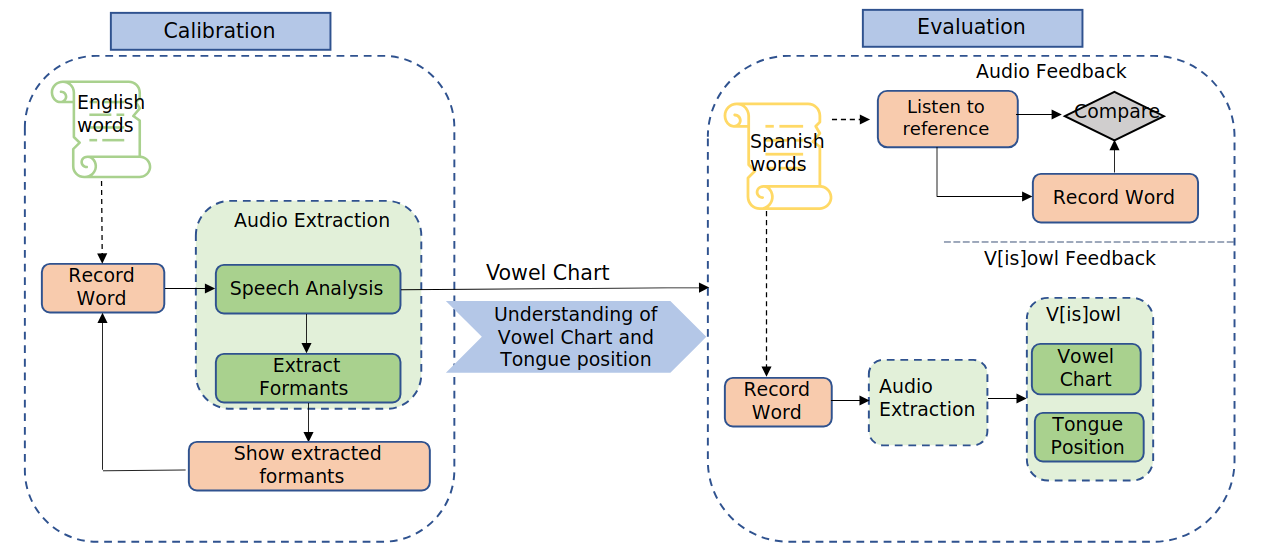
\includegraphics[width=0.8\linewidth]{pictures/workflows/flowPractice.png}
    \caption{The study begins by calibrating a user's voice using extracted formants of four English vowels [\textipa{i},u,a,\textipa{6}]. After calibration, users interact with an audio-only feedback system and \visowel{}, which extracts formants and displays them on a vowel chart. }
    \label{fig:workflowPrac}
\end{figure*}



% \subsection{Visual Feedback for Audio Signals}
% \todo{write this section :)}

\subsection{Research Questions}
As we seek to understand what makes a visualization effective, we need to make sure we view it holistically. If a visualization is effective in improving the target sounds, such as vowels, but does not affect or negatively affects overall pronunciation, we should consider visualizations that communicate information for more sounds. In short, to understand what makes visualizations effective and if they limit speakers during practice, we seek to answer the following questions:

\begin{itemize}
    \item[\textbf{RQ1:}] How does interaction between a visual and audio-only feedback method differ?
    \item[\textbf{RQ2:}] How do phonetically untrained users interpret vowel charts during interaction?
    \item[\textbf{RQ3:}] How does a visualization that focuses on vowels affect users' perceptions of other aspects of pronunciation?
\end{itemize}
% Because it is not clear what aspects of visualizations learners find useful during practice, we ask questions that help us know how users interpret the visual feedback. 
% Research indicates that higher motivation in language learning correlates with commitment to learning a language; the longer one learns a language the better the pronunciation becomes.


% In general, studies show that immediate explicit pronunciation feedback is beneficial for L2 learners~\cite{darcy2021window,lacabex_explicit_2020,yakut_promoting_2020, sepasdar_immediate_2019}.

% \footnote{A monophthong is one sound and a diphthong is the blending of two sounds, for example, "I" in English is generally said as a diphthong.}